\section{Analysis of Murders in Sicily: a Point Process Perspective}

In collaboration with the Prosecutor's Office of Palermo, last year I started working on a project that focused on the study of data concerning murders, attempted murders and disappearances in Sicily. We were able to build a dataset of about 5000 events, spanning from 1945 to 2025, with information about the victim and the date of the event; in about 70\% of the cases, we also have information about the location of the event.

This dataset is particularly valuable, as the events can be considered a proxy for the activity of Mafia in Sicily. Last year I was able to perform a preliminary analysis of the data, focusing on the temporal and spatial distribution of the events. The analysis showed that, from a temporal perspective, the data shows a bursty pattern, with clusters of events occurring in short time frames followed by periods of relative calm, in a dynamics that is reminiscent of earthquake occurrences.

This year I focused on modeling the phenomenon as a \textbf{point process} in time. This approach is common in seismology, where earthquakes are modeled as points in time and space (ETAS model), in finance, in neuroscience, and was used also in the analysis of crime data \cite{mohlerSelfExcitingPointProcess2011,bacryHawkesProcessesFinance2015,laubElementsHawkesProcesses2021}.

Formally, a point process $\{T_i\}_{i \in \mathbb{N}}$ is a random collection of points on a measurable space, typically $\mathbb{R}$ for temporal processes. The \textit{arrival times} $T_i$ can be independent of each other, as in a Poisson process, or they can exhibit dependencies, as in a \textbf{self-exciting process} or \textbf{Hawkes process}. This latter case is particularly interesting, as it captures the phenomenon where the occurrence of an event increases the likelihood of subsequent events in the near future, leading to clustering behavior similar to what we observed in the data.

In a point process, it is common to define the \textbf{conditional intensity function} $\lambda(t | \mathcal{H}_t)$, which represents the instantaneous rate of occurrence of events at time $t$, given the history $\mathcal{H}_t$ of the process up to time $t$. For a Hawkes process, the conditional intensity function can be expressed as:
\begin{equation}
  \lambda(t | \mathcal{H}_t) = \mu + \sum_{T_i < t} g(t - T_i)
\end{equation}
where $\mu$ is the baseline intensity (the rate of events in the absence of self-excitation), and $g(t - T_i)$ is a triggering function that quantifies the influence of past events $T_i$ on the current intensity. A common choice for the triggering function is an exponential decay function:
\begin{equation}
  g(t - T_i) = \alpha e^{-\beta (t - T_i)}
\end{equation}
where $\alpha > 0$ controls the magnitude of the influence and $\beta > 0$ controls the decay rate. In this formulation the expected number of events triggered by a single event, known as \textbf{branching ratio}, is given by $\frac{\alpha}{\beta}$.

Given some observed data it's possible to \textit{infer} the parameters of the model: the most common frameworks are \textit{Maximum Likelihood Estimation} (MLE), \textit{Moment Matching}, \textit{Expectation-Maximization} (EM), and \textit{Bayesian Inference} \cite{laubElementsHawkesProcesses2021}.

In the case of the murders dataset the arrival times are known with only daily resolution: this kind of lack of information is called \textbf{interval censoring} \cite{laubElementsHawkesProcesses2021} in the point process literature, and it poses challenges for parameter estimation, as the actual arrival times are not observed, and a simple Maximum Likelihood Estimation (MLE) approach cannot be directly applied.

Many approaches can be used to address this issue, such as data augmentation techniques, where the unobserved arrival times are treated as latent variables and estimated alongside the model parameters using EM \cite{shlomovichParameterEstimationMethod2022} or Bayesian methods \cite{derektuckerHandlingMissingData2019}. A simpler approach is given by using a moment matching method that accounts for the censoring in the data \cite{laubElementsHawkesProcesses2021} or by jittering the arrival times within their known intervals.

By applying this latter approach on the most intense period (events from 1975 to 2000), I was able to fit the simple exponential univariate Hawkes model to the data. The branching ratio is about 0.4, indicating a significant level of self-excitation in the data. The goodness of fit can be evaluated by the CCDF of the inter-event times and by looking at the QQ-plot of the transformed inter-event times \cite{laubElementsHawkesProcesses2021}, as in \autoref{fig:hawkes-ccdf} and \autoref{fig:hawkes-qq}.

\begin{figure}[H]
    \centering
    \begin{subfigure}[t]{.49\textwidth}
        \centering
        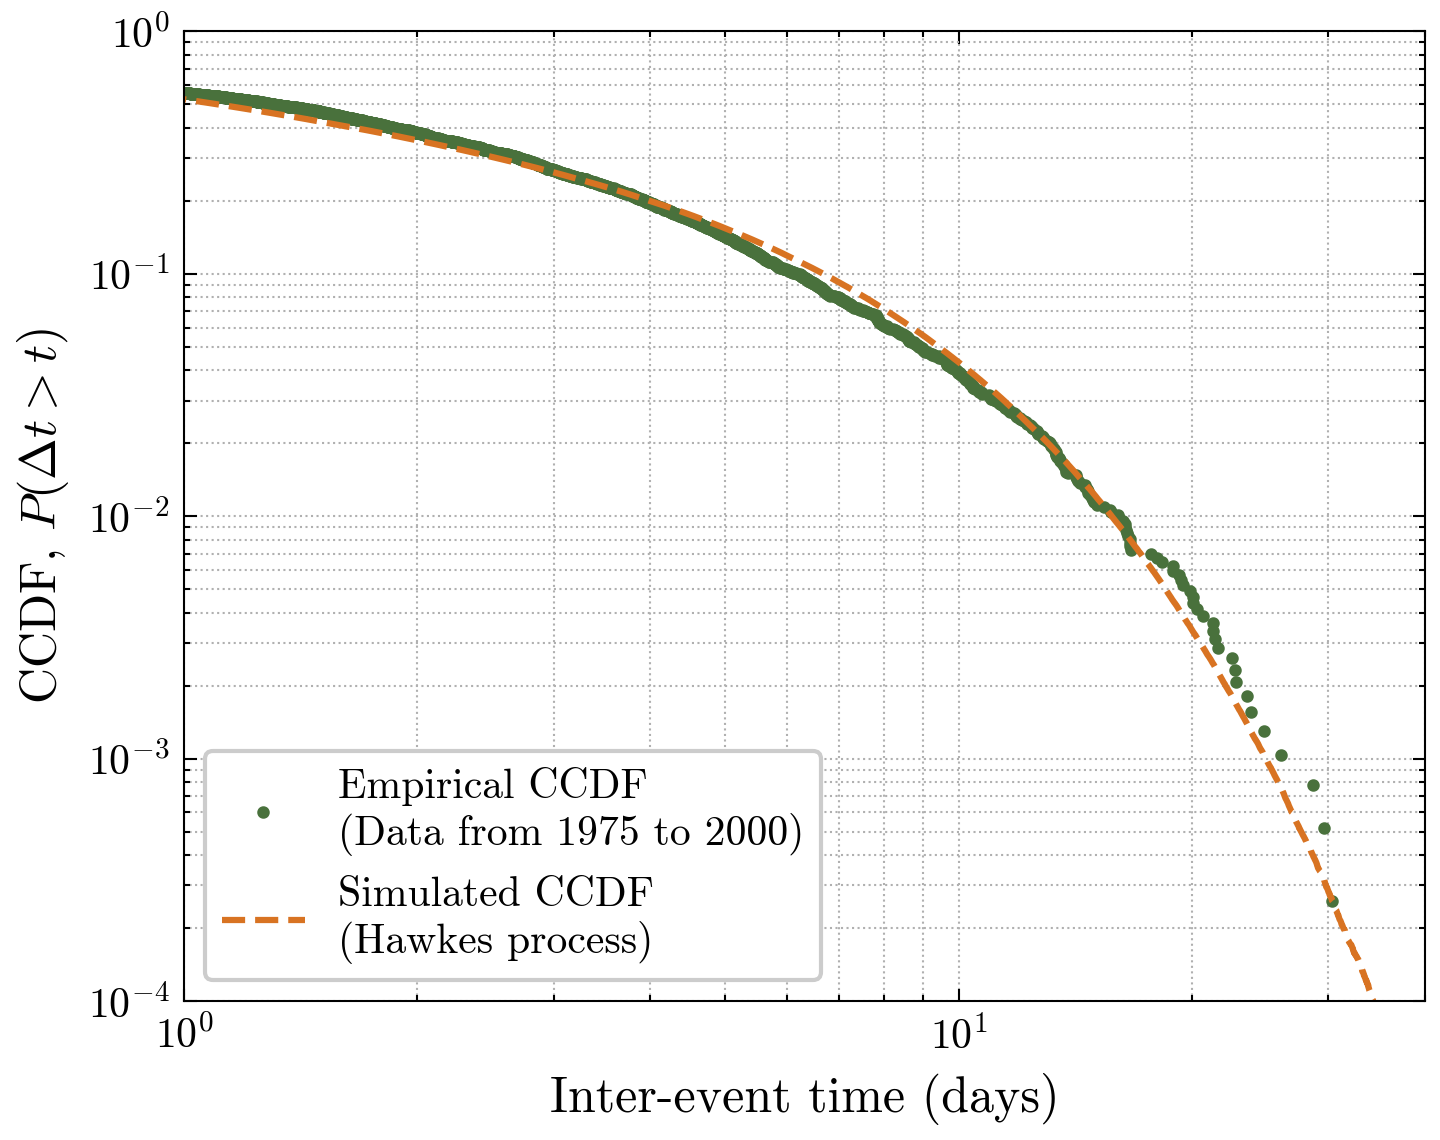
\includegraphics[width=\textwidth]{figures/hawkes-ccdf.png}
        \caption{CCDF of inter-event times in log-log scale}
        \label{fig:hawkes-ccdf}
    \end{subfigure}%
    \hspace{1em}
    \begin{subfigure}[t]{.47\textwidth}
        \centering
        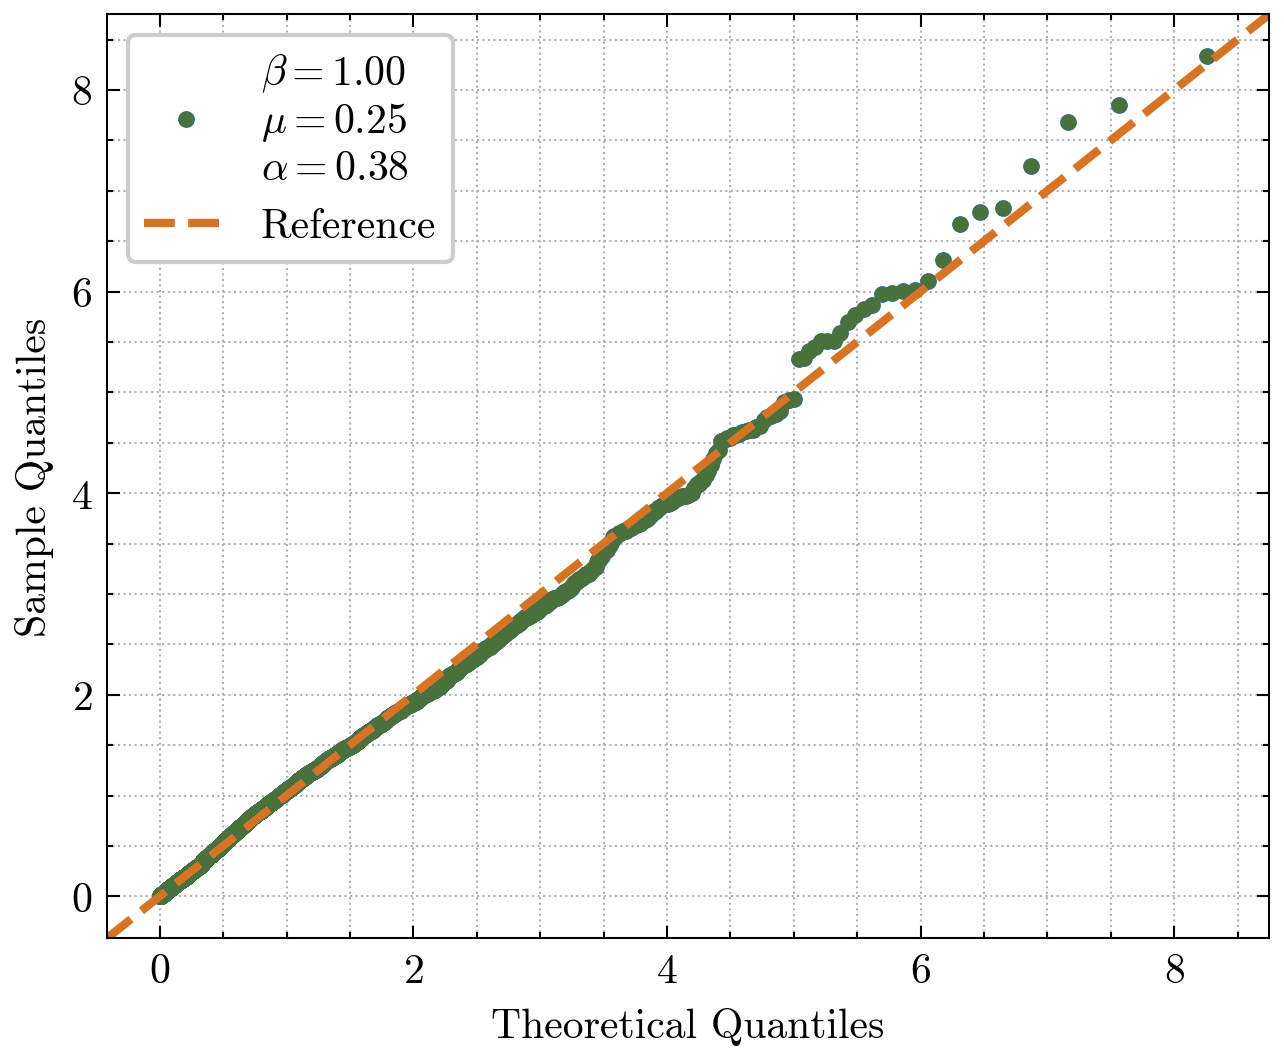
\includegraphics[width=\textwidth]{figures/hawkes-qq.png}
        \caption{QQ plot of inter-event times transformed via time-rescaling theorem with the fitted Hawkes model}
        \label{fig:hawkes-qq}
    \end{subfigure}
    \caption{Simulated vs empirical inter-event times for the fitted Hawkes model on murders in Sicily (1975-2000). The good agreement indicates a good fit of the model to the data.}
\end{figure}

The good fit of this simple model suggests that the process is self-exciting in nature: the occurrence of a murder increase the likelihood of a subsequent murder, for example because of retaliation. The model is a valid starting point for more complex analyses with different functional forms for the triggering function, incorporating also the spatial information.

